%
% Template Laporan Skripsi/Thesis 
%
% @author  Andreas Febrian, Lia Sadita 
% @version 1.03
%
% Dokumen ini dibuat berdasarkan standar IEEE dalam membuat class untuk 
% LaTeX dan konfigurasi LaTeX yang digunakan Fahrurrozi Rahman ketika 
% membuat laporan skripsi. Konfigurasi yang lama telah disesuaikan dengan 
% aturan penulisan thesis yang dikeluarkan UI pada tahun 2008.
%

%
% Tipe dokumen adalah report dengan satu kolom. 
%
\documentclass[12pt, a4paper, onecolumn, oneside, final]{report}

% Load konfigurasi LaTeX untuk tipe laporan thesis
\usepackage{_internals/uithesis}

% Daftar pemenggalan suku kata dan istilah dalam LaTeX
%
% Hyphenation untuk Indonesia 
%
% @author  Andreas Febrian
% @version 1.00
% 
% Tambahkan cara pemenggalan kata-kata yang salah dipenggal secara otomatis 
% oleh LaTeX. Jika kata tersebut dapat dipenggal dengan benar, maka tidak 
% perlu ditambahkan dalam berkas ini. Tanda pemenggalan kata menggunakan 
% tanda '-'; contoh:
% menarik
%   --> pemenggalan: me-na-rik
%

\hyphenation{
    % alphabhet A
    a-na-li-sa a-tur 
    a-pli-ka-si 
    % alphabhet B
    ba-ngun-an 
    be-be-ra-pa 
    ber-ge-rak
    ber-ke-lan-jut-an 
    ber-pe-nga-ruh 
    % alphabhet C
    ca-ri
    % alphabhet D
    di-sim-pan di-pim-pin de-ngan da-e-rah di-ba-ngun da-pat di-nya-ta-kan 
    di-sim-bol-kan di-pi-lih di-li-hat de-fi-ni-si
    % alphabhet E
    e-ner-gi eks-klu-sif
    % alphabhet F
    fa-si-li-tas
    % alphabhet G
    ga-bung-an ge-rak
    % alphabhet H
    ha-lang-an
    % alphabhet I
    % alphabhet J
    % alphabhet K
    ke-hi-lang-an
    ku-ning 
    kua-li-tas ka-me-ra ke-mung-kin-an ke-se-pa-ham-an
    % alphabhet L
    ling-kung-an
    % alphabhet M
    me-neng-ah
    meng-a-tas-i me-mung-kin-kan me-nge-na-i me-ngi-rim-kan 
    meng-u-bah meng-a-dap-ta-si me-nya-ta-kan mo-di-fi-ka-si
    meng-a-tur
    % alphabhet N
    nya-ta non-eks-klu-sif
    % alphabhet O
    % alphabhet P
	pe-nye-rap-an 
	pe-ngon-trol
    pe-mo-del-an
    pe-ran  pe-ran-an-nya
    pem-ba-ngun-an pre-si-den pe-me-rin-tah prio-ri-tas peng-am-bil-an 
    peng-ga-bung-an pe-nga-was-an pe-ngem-bang-an 
    pe-nga-ruh pa-ra-lel-is-me per-hi-tung-an per-ma-sa-lah-an 
    pen-ca-ri-an peng-struk-tur-an
    % alphabhet Q
    % alphabhet R
    ran-cang-an
    % alphabhet S
    si-mu-la-si sa-ngat
    % alphabhet T
    te-ngah
    ter-da-pat
    % alphabhet U
    % alphabhet V
    % alphabhet W
    % alphabhet X
    % alphabhet Y
    % alphabhet Z
    % special
}

% Load konfigurasi khusus untuk laporan yang sedang dibuat
%-----------------------------------------------------------------------------%
% Informasi Mengenai Dokumen
%-----------------------------------------------------------------------------%
% 
% Judul laporan. 
\var{\judul}{Judul Skripsi/Thesis/Disertasi}
% 
% Tulis kembali judul laporan, kali ini akan diubah menjadi huruf kapital
\Var{\Judul}{Judul Skripsi/Thesis/Disertasi}
% 
% Tulis kembali judul laporan namun dengan bahasa Ingris
\var{\judulInggris}{Unknown Title for Final Report/Thesis/Disertation}

% 
% Tipe laporan, dapat berisi Skripsi, Tugas Akhir, Thesis, atau Disertasi
\var{\type}{Skripsi}
% 
% Tulis kembali tipe laporan, kali ini akan diubah menjadi huruf kapital
\Var{\Type}{Skripsi}
% 
% Tulis nama penulis 
\var{\penulis}{Nama Penulis}
% 
% Tulis kembali nama penulis, kali ini akan diubah menjadi huruf kapital
\Var{\Penulis}{Nama Penulis}
% 
% Tulis NPM penulis
\var{\npm}{NPM}
% 
% Tuliskan Fakultas dimana penulis berada
\Var{\Fakultas}{Ilmu Komputer}
\var{\fakultas}{Ilmu Komputer}
% 
% Tuliskan Program Studi yang diambil penulis
\Var{\Program}{ILMU KOMPUTER}
\var{\program}{Ilmu Komputer}
% 
% Tuliskan tahun publikasi laporan
\Var{\bulan}{Juli}
\Var{\tahun}{2019}
% 
% Tuliskan gelar yang akan diperoleh dengan menyerahkan laporan ini
\var{\gelar}{Sarjana Ilmu Komputer}
% 
% Tuliskan tanggal pengesahan laporan, waktu dimana laporan diserahkan ke 
% penguji/sekretariat
\var{\tanggalPengesahan}{XX Juli 2019} 
% 
% Tuliskan tanggal keputusan sidang dikeluarkan dan penulis dinyatakan 
% lulus/tidak lulus
\var{\tanggalLulus}{XX Juli 2019}
% 
% Tuliskan pembimbing 
\var{\pembimbing}{Prof. ???}
% 
% Alias untuk memudahkan alur penulisan paa saat menulis laporan
\var{\saya}{Penulis}

%-----------------------------------------------------------------------------%
% Judul Setiap Bab
%-----------------------------------------------------------------------------%
% 
% Berikut ada judul-judul setiap bab. 
% Silahkan diubah sesuai dengan kebutuhan. 
% 
\Var{\kataPengantar}{Kata Pengantar}
\Var{\babSatu}{Pendahuluan}
\Var{\babDua}{Sekilas Mengenai \latex}
\Var{\babTiga}{Notasi Matematik}
\Var{\babEmpat}{Struktur Berkas}
\Var{\babLima}{Perintah dalam uithesis.sty}
\Var{\babEnam}{Bab Enam}
\Var{\kesimpulan}{Kesimpulan dan Saran}

% Daftar istilah yang mungkin perlu ditandai 
%
% @author  Andreas Febrian
% @version 1.00
% 
% Mendaftar seluruh istilah yang mungkin akan perlu dijadikan 
% italic atau bold pada setiap kemunculannya dalam dokumen. 
% 

\var{\license}{\f{Creative Common License 1.0 Generic}}
\var{\bslash}{$\setminus$}

% Awal bagian penulisan laporan
\begin{document}
%
% Sampul Laporan
%
% Sampul Laporan

%
% @author  unknown
% @version 1.01
% @edit by Andreas Febrian
%

\begin{titlepage}
    \begin{center}    
        \begin{figure}
            \begin{center}
                
\includegraphics[width=2.5cm]{_internals/makara.eps}
            \end{center}
        \end{figure}    
        \vspace*{0cm}
        \bo{
        	UNIVERSITAS INDONESIA\\
        }
        
        \vspace*{1.0cm}
        % judul thesis harus dalam 14pt Times New Roman
        \bo{ANALISIS FAKTOR-FAKTOR PENGARUH VARIASI KONSENTRASI
        LAPISAN OZON STRATOSFER DENGAN REGRESI} \\[1.0cm]

        \vspace*{2.5 cm}    
        % harus dalam 14pt Times New Roman
        \bo{LAPORAN AKHIR KULIAH PEMODELAN MATEMATIS \\ SEMESTER GANJIL 2022} \\
        [1.0cm]

        \vspace*{3 cm}       
        % penulis dan npm
       \bo{ Agustinus Bravy Tetuko Ompusunggu​ (2006521300)\\
Antonius Rangga Hapsoro Wicaksono​ (2006568790​)\\
Carles Octavianus​ (2006568613)\\
Fenny Fadhilah Zakiyyatunnisa (2006568853)\\
Rafaella Garcinia Gayatri (2006572226)\\
Yohanes Bryan Sagala (2006568696) \\
}

        \vspace*{2.5cm}

        % informasi mengenai fakultas dan program studi
        \bo{
        	FAKULTAS MATEMATIKA DAN ILMU PENGETAHUAN ALAM
        	PROGRAM STUDI MATEMATIKA \\
        	DEPOK \\
        	2023
        }
    \end{center}
\end{titlepage}


%
% Gunakan penomeran romawi
\pagenumbering{roman}
%
% setelah bagian ini, halaman dihitung sebagai halaman ke 2
\setcounter{page}{2}
%
%
\addChapter{\kataPengantar}
%-----------------------------------------------------------------------------%
\chapter*{Kata Pengantar}
%-----------------------------------------------------------------------------%

Puji syukur kehadirat Tuhan Yang Maha Esa karena rahmat dan anugerah-Nya telah memberikan kesempatan pada penulis untuk menyelesaikan makalah ini. Atas rahmat dan anugerah-Nya lah penulis dapat menyelesaikan makalah yang berjudul ‘Analisis Faktor-Faktor Pengaruh Variasi  Konsentrasi Lapisan Ozon Stratosfer dengan Regresi Linear’ secara tepat waktu.

Makalah ‘Analisis Faktor-Faktor Pengaruh Variasi Konsentrasi Lapisan Ozon Stratosfer dengan Regresi Linear’ disusun guna memenuhi tugas akhir mata kuliah pemodelan matematis dengan dosen pembimbing Bapak Dr. Hengki Tasman, S.Si., M.Si. di Universitas Indonesia. Selain itu, penulis juga berharap agar makalah ini dapat menambah wawasan bagi pembaca tentang analisis faktor-faktor pengaruh variasi konsentrasi lapisan ozon.

Penulis mengucapkan terima kasih sebesar-besarnya kepada Bapak Dr. Hengki Tasman, S.Si., M.Si. selaku dosen pembimbing penulis pada mata kuliah pemodelan matematis. Tugas yang telah diberikan ini dapat menambah pengetahuan dan wawasan terkait bidang yang ditekuni penulis. Penulis juga mengucapkan terima kasih pada seluruh dosen mata kuliah pemodelan matematis dan semua pihak yang telah membantu proses penyusunan makalah ini.

Penulis menyadari makalah ini masih jauh dari kata sempurna. Oleh karena itu, kritik dan saran yang membangun akan penulis terima demi kesempurnaan makalah ini.


\vspace*{0.2cm}
\begin{flushright}
Depok, 06 Januari 2023 \\[0.1cm]
\vspace*{1.5cm}
\\Kelompok Ozon

\end{flushright}
%
% 
\addChapter{ABSTRAK}
%
% Halaman Abstrak
%
% @author  Andreas Febrian
% @version 1.00
%

\chapter*{Abstrak}

\vspace*{0.2cm}
{
	\setlength{\parindent}{0pt}
	
	\begin{tabular}{@{}l l p{10cm}}
		Nama&: & Kelompok Ozon \\
		Program Studi&: & Matematika \\
		Judul&: & Analisis Faktor-Faktor Pengaruh Variasi  Konsentrasi Lapisan Ozon Stratosfer dengan Regresi Linear \\
		Pembimbing&: & Dr. Hengki Tasman, S.Si., M.Si. \\
	\end{tabular}

	\bigskip
	\bigskip
    Makalah ini membahas Analisis Faktor-Faktor Pengaruh Variasi  Konsentrasi Lapisan Ozon Stratosfer dengan Regresi Linear Penelitian ini adalah penelitian kuantitatif dengan desain deskriptif. Hasil penelitian didapatkan bahwa variasi konsentrasi lapisan ozon dipengaruhi oleh beberapa faktor, dan faktor-faktor yang memengaruhinya juga bergantung pada lokasi penelitian dan juga rentang waktu penelitian. 

	\bigskip

	Kata kunci:\\
	Faktor, Lapisan Ozon, Regresi
}

\newpage
%
%
\phantomsection
\tableofcontents
\clearpage
\phantomsection
\listoffigures
\clearpage
\phantomsection
\listoftables
\clearpage

%
% Gunakan penomeran Arab (1, 2, 3, ...) setelah bagian ini.
%
\pagenumbering{arabic}

%
%
%
%-----------------------------------------------------------------------------%
\chapter{Pendahuluan}
%-----------------------------------------------------------------------------%
%-----------------------------------------------------------------------------%
\section{Latar Belakang}
%-----------------------------------------------------------------------------%
Lapisan ozon adalah wilayah stratosfer Bumi yang mengandung konsentrasi ozon (O3) tinggi dibandingkan di lapisan lain. Lapisan ozon utamanya ditemukan di bagian bawah stratosfer, dari sekitar 15 hingga 35 kilometer (9 hingga 22 mil) di atas Bumi. Ketebalan lapisan ozon bervariasi secara musiman dan geografis.

Lapisan ozon berperan penting sebagai penyerap radiasi ultraviolet Matahari. Lapisan ozon menyerap 97 hingga 99 persen sinar ultraviolet frekuensi menengah Matahari (dari panjang gelombang sekitar 200 nm hingga 315 nm). Jika tidak diserap, sinar ini berpotensi merusak kehidupan di permukaan Bumi.

\textit{Ozone depletion} adalah fenomena penipisan (pemecahan) ozon pada lapisan ozon di bumi yang disebabkan oleh \textit{ozone depleting substances}. \textit{Ozone-depleting substances} (ODS) adalah gas halogen yang memuat klorin dan/atau bromin yang mempunyai potensi untuk memecah ozon di stratosfer. Beberapa contoh dari ODS antara lain klorofluorokarbon (CFC), hidroklorofluorokarbon (HCFC), metil klorida, metil bromida, dan halon. \textit{Ozone-depleting substances} dapat disebabkan secara natural dan antropogenik.

Proses yang dapat memengaruhi variasi konsentrasi lapisan ozon antara lain, \textit{Midlatitude Halogen Chemistry}, \textit{Aerosol Effects}, \textit{Quasi-Biennial Oscillation}, \textit{Solar Cycle}.



%-----------------------------------------------------------------------------%
\section{Permasalahan}
%-----------------------------------------------------------------------------%
Pada bagian ini akan dijelaskan mengenai rumusan masalah 
yang \saya~hadapi dan ingin diselesaikan serta asumsi dan batasan 
yang digunakan dalam menyelesaikannya.


%-----------------------------------------------------------------------------%
\subsection{Rumusan Masalah}
%-----------------------------------------------------------------------------%
\begin{enumerate}
    \item Apa saja faktor-faktor yang memengaruhi variasi konsentrasi lapisan ozon?
    \item Bagaimana model matematis untuk mengkuantifikasi pengaruh masing-masing faktor terhadap variasi konsentrasi lapisan ozon?
\end{enumerate}


%-----------------------------------------------------------------------------%
\subsection{Batasan Permasalahan}
%-----------------------------------------------------------------------------%
Pada penelitian ini penulis tidak menggunakan model untuk prediksi, melainkan penulis hanya memodelkan untuk interpretasi supaya dapat menentukan faktor-faktor yang memengaruhi variasi konsentrasi lapisan ozon.


%-----------------------------------------------------------------------------%
\section{Tujuan}
%-----------------------------------------------------------------------------%
\begin{enumerate}
    \item Mengetahui faktor-faktor yang memengaruhi variasi konsentrasi lapisan ozon
    \item Membangun model matematis untuk mengkuantifikasi pengaruh masing-masing faktor terhadap variasi konsentrasi lapisan ozon
\end{enumerate}

%-----------------------------------------------------------------------------%
\section{Metodologi Penelitian}
%-----------------------------------------------------------------------------%
Metodologi penelitian yang penulis gunakan adalah metode kuantitatif dengan desain deskriptif.


%-----------------------------------------------------------------------------%
\chapter{Pembahasan}

\section{Landasan Teori}
%-----------------------------------------------------------------------------%
\subsection{Ketebalan Ozon}
Ozon adalah molekul gas yang tersusun dari tiga atom oksigen yang secara alami terdapat di atmosfer bumi dan menyerap radiasi sinar ultraviolet pada panjang gelombang tertentu. Ozon terdapat di seluruh atmosfer, tetapi sebagian besar terdapat di lapisan stratosfer. Ozon inilah yang dikenal dengan istilah “Lapisan Ozon”. \\~\\
Secara alamiah ozon tersebar dalam stratosfer
membentuk lapisan yang tebalnya kurang lebih 35 km. Konsentrasi ozon di lapisan stratosfer bervariasi menurut ketinggian.Lapisan ozon yang tipis ini apabila
dibandingkan dengan tebalnya seluruh atmosfer bumi cukup
efisien dalam menyaring semua sinar ultraviolet matahari yang
berbahaya bagi makhluk hidup di bumi. Oleh karena itu, ozon
penting sekali bagi kehidupan di muka bumi dari bahaya
sengatan ultraviolet. \\~\\
Ketebalan lapisan ozon di stratosfer dapat diukur dengan sebuah alat yang bernama Spektrofotometer Dobson dan satuan yang digunakan untuk mengukur ketebalan lapisan ozon adalah Dobson Unit (DU), dimana 1 DU adalah jumlah molekul ozon yang dibutuhkan untuk membentuk satu lapisan ozon setebal 0,01 mm pada suhu 0$^{\circ}$C dan tekanan 1 atm.

\subsection{Fenomena yang Berpotensi Mempengaruhi Ketebalan Ozon}

Ozon terbentuk secara alami melalui siklus Chapman, dimana reaksi pemecahan molekul Oksigen (O2) oleh sinar UV menjadi dua atom oksigen yang kemudian bereaksi dengan molekul oksigen lain menjadi molekul O3. Pembentukan molekul ozon paling banyak terbentuk di daerah tropis karena intensitas sinar UV paling optimum di daerah tersebut.

\begin{figure}[h!]
    \centering
    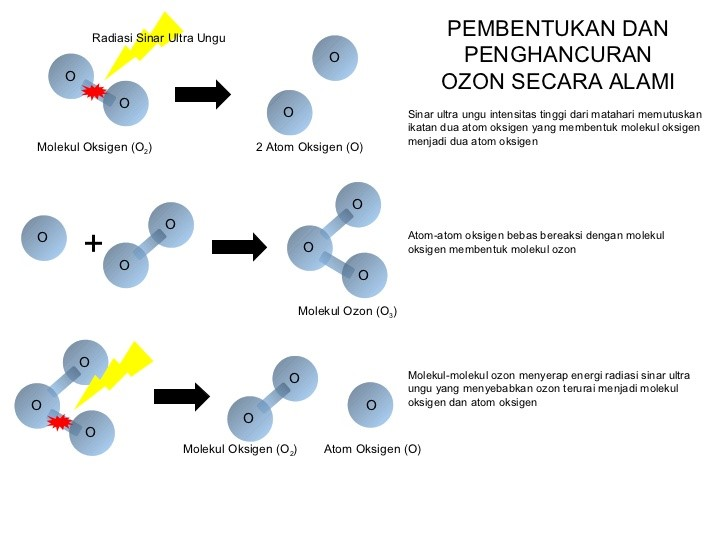
\includegraphics[scale=0.7]{src/Pics/PROSES PEMBENTUKAN OZON SECARA ALAMI.jpg}
    \caption{Proses Pembentukan Ozon Secara Alami}
    \label{fig:my_label}
\end{figure}\\~\\
Secara alami, ozon bereaksi dengan berbagai molekul yang mengandung nitrogen, hidrogen dan klorin. Jumlah molekul-molekul tersebut sangatlah kecil sehingga tidak mengganggu kelimpahan ozon di stratosfer. 
Kelimpahan ozon akan terganggu oleh \textit{Ozone Depleting Substances} (ODS) yang merupakan senyawa kimia yang terdiri dari unsur karbon, hidrogen, klorin dan/atau bromin.  Senyawa tersebut tidak mudah terurai pada lapisan atmosfer bawah (troposfer) dan bersifat sangat stabil. Sebagai contoh, ODS banyak digunakan dalam peralatan pendingin buatan manusia (refrigeran), contohnya senyawa CFC \textit{(chlorofluorocarbon)} yang mengandung klorin. Klorin yang terlepas dari CFC akan menguraikan ikatan O3, sehingga kerapatan lapisan ozon akan berkurang jika proses tersebut berlanjut. Dari fenomena ini, penipisan lapisan ozon terjadi.
\begin{figure}[h!]
    \centering
    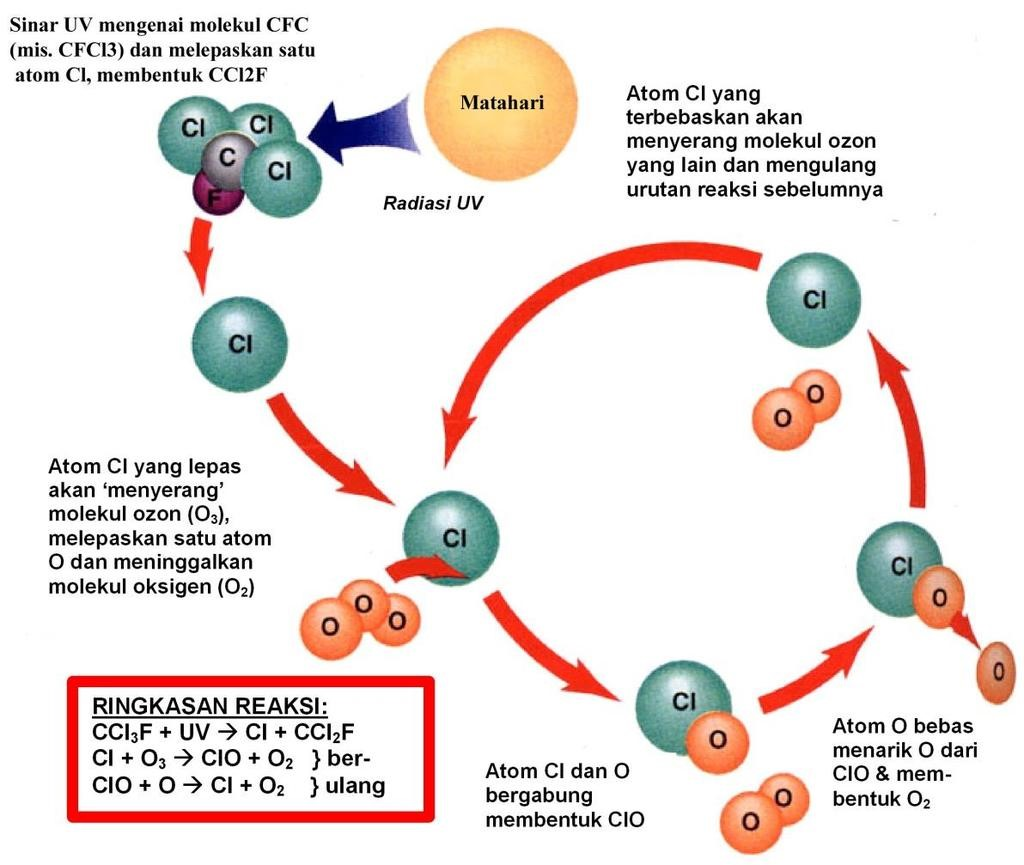
\includegraphics[scale=0.3]{src/Pics/PROSES PERUSAKAN OZON DI LAPISAN STRATOSFER.jpg}
    \caption{Proses Perusakan Ozon di Lapisan Stratosfer}
    \label{fig:my_label}
\end{figure}\\~\\
Fenomena adanya pengaruh ODS di atmosfer dapat memengaruhi ketebalan lapisan ozon menipis, padahal ozon pada lapisan stratosfer berfungsi sebagai filter
sekaligus pelindung bumi dari pengaruh berbahaya radiasi matahari.
Radiasi ultraviolet (UV) yang berasal dari matahari berbahaya bagi kehidupan di
bumi. Meningkatnya jumlah radiasi UV (UV-B) dapat merusak rantai
makanan yang ada di laut. Di samping itu, terdapat hubungan yang kuat antara
meningkatnya UV dengan meningkatnya kasus-kasus penyakit kanker kulit dan
katarak mata pada manusia. Pada dasarnya atmosfer bertindak sebagai perisai
terhadap radiasi matahari melalui penyebaran atau penyerapan oleh molekul-
molekul gas yang ada di dalam atmosfer bumi. Dalam hal ini, ozonlah yang paling
efektif menyerap radiasi UV. Secara alami molekul-molekul ozon terbentuk dan
rusak di atmosfer bumi. Secara alami pula penipisan lapisan ozon terjadi di atas
kutub selatan setiap musim semi.

\subsection{Variabel Proxy}
\begin{enumerate}
    \item EESC \textit{(Equivalent Effective Stratospheric Chlorine)}\\
Gas sumber halogen yang berkontribusi terhadap penipisan ozon sebagian besar adalah bahan kimia yang mengandung klorin dan bromin yang memiliki masa hidup yang sangat lama di atmosfer. EESC adalah parameter yang mudah digunakan untuk memperkirakan jumlah penipisan ozon stratosfer karena senyawa tersebut. Semakin tinggi nilai EESC, semakin banyak klorin tersedia untuk penghancuran ozon. Satuan EESC adalah \textit{parts per billion by volume} (ppbv, volume klorin setara dengan volume udara).

EESC merupakan proxy yang digunakan pada \textit{Midlatitude Halogen Chemistry}, yaitu reaksi kimia zat halogen yang terjadi pada \textit{midlatitudes} (daerah yang berada di antara 35 hingga 55 derajat lintang selatan maupun utara. Pada lintang ini, terjadi reaksi halogen karena adanya zat halogen bebas akibat reaksi \textit{photochemical} dan reaksi heterogen yang disebabkan oleh \textit{volcanic sulfate aerosols}. Zat halogen yang terdapat pada lintang ini adalah Cl dan Br, di mana kedua senyawa ini akan mengganggu pembentukan zat-zat yang membentuk lapisan ozon.

    \item \textit{Solar Flux} \\
\textit{Solar flux} merupakan \textit{proxy variable} yang digunakan untuk merepresentasikan proses \textit{solar cycle}. \textit{Solar cycle} adalah siklus perubahan besarnya radiasi matahari dengan besar periode sekitar 11 tahun. Matahari kita adalah bola gas panas bermuatan listrik yang sangat besar. Gas bermuatan ini bergerak, menghasilkan medan magnet yang kuat. Medan magnet Matahari melewati sebuah siklus, yang disebut siklus matahari.

    \item QBO \textit{(Quasi-biennial Oscillation)} \\
\textit{Quasi-biennial Oscillation} (QBO) adalah variasi iklim secara berkala yang diidentifikasi berdasarkan pola angin atau massa udara yang berhembus pada lapisan stratosfer di atas ekuator yang ditandai oleh fenomena berputarnya angin tropikal di stratosfer bawah dari arah timur ke arah barat yang terjadi dalam waktu dua tahun sekali. Perputaran ini akan mempengaruhi transpor ozon. Bila di stratosfer berhembus angin baratan maka ozon pada lintang menengah dan kutub akan berkurang sekitar 6\% – 8\%. Sebaliknya, bila angin timuran  berhembus akan meningkatkan konsentrasi ozon. Massa udara tersebut menjalar mengelilingi bumi sepanjang ekuator dan setiap 14 bulan atau lebih, arahnya akan berbalik menuju arah yang berlawanan. Dengan demikian, total dalam 1 siklus pada arah timuran dan baratan kemudian kembali ke timuran, QBO membutuhkan waktu sekitar 28 bulan. Dua proxy digunakan untuk menjelaskan kemungkinan pergeseran fasa sementara dari sinyal QBO, yaitu QBO-30 dan QBO-50.

    \item \textit{Aerosol Backscatter Ratio}\\
\textit{Aerosol Backscatter Ratio} (ABR) merupakan \textit{proxy variable} yang digunakan untuk merepresentasikan jumlah zat aerosol yang berada dalam atmosfer. Untuk pengukurannya sendiri dilakukan dengan menggunakan LiDAR, yaitu sensor cahaya yang memancarkan sinar ke daerah tertentu dan mengolah sinar yang terpantulkan kembali untuk memperoleh informasi tentang hal tersebut. Fenomena terpantulnya kembali cahaya ke sensor disebut \textit{backscattering}. \textit{Backscattering} dipengaruhi oleh sifat zat yang sedang diteliti, antara lain ukuran partikel dan ketebalan. Oleh karena itu, atmosfer yang tidak mengandung aerosol akan menghasilkan backscattering yang berbeda dengan atmosfer yang mengandung aerosol.
Rasio dari kemampuan \textit{backscattering} atmosfer yang mengandung aerosol dengan kemampuan \textit{backscattering} atmosfer biasa (tidak mengandung aerosol) disebut \textit{aerosol backscatter ratio}.

    \item \textit{Column Ozone} \\
TCO \textit{(Total Column Ozone)} yaitu \textit{proxy variable} untuk pengukuran jumlah total ozon atmosfer dalam kolom tertentu. Biasanya, TCO diukur dalam Dobson Units (DU), dimana 1 DU adalah jumlah molekul ozon yang dibutuhkan untuk membentuk satu lapisan ozon setebal 0,01 mm pada suhu 0$^{\circ}$C dan tekanan 1 atm.



%-----------------------------------------------------------------------------%
\section{Metode Statistik}
\subsection{Regresi Linear}
Regresi Linear merupakan metode pembentukan model prediksi. Tujuan dari model ini adalah untuk mengekspresikan relasi terhadap variabel dependen $y \in R^n$ terhadap satu atau lebih variabel independen $X_i \in R^n$. Model yang diperoleh dapat digunakan untuk memprediksi nilai $y$ berdasarkan variabel - variabel independen yang dimiliki. Contoh model regresi linear:
\begin{equation*}
    Y = \beta_1X_1 + \beta_2X_2 + \ldots + \beta_iX_i + \epsilon,\;\epsilon \sim N(0, \sigma^2)
\end{equation*}
Dengan varibel $a_i$ merepresentasikan parameter atau koefisien untuk setiap variabel $X_i$
\subsection{Statistik Model Regresi}\label{Statistik Model Regresi}
% List yang harus dijelasin
\begin{enumerate}
    \item Korelasi Pearson ($r$) \\
    Tipe korelasi yang menjelaskan hubungan antar dua variabel, misal $x$ dan $y$. Koefisien Pearson memiliki \textit{range} nilai -1 sampai dengan 1. \\
    Koefisien Pearson didapat dengan:
    \begin{equation*}
        r = \frac{\sum (X_i - \overline{x})(y_i - \overline{y})}{\sqrt{\sum (X_i - \overline{x})^2(y_i - \overline{y})^2}}
    \end{equation*}
    Dengan:
    \begin{itemize}
        \item $r$ = Koefisien Pearson
        \item $X_i$ = nilai ke-i variabel $x$
        \item $\overline{x}$ = Nilai rata - rata variabel x
        \item $y_i$ = nilai ke-i variabel $y$
        \item $\overline{y}$ = Nilai rata - rata variabel y
    \end{itemize}
    Interpretasi nilai $r$:
    \begin{itemize}
        \item Bila korelasi $r$ berada pada \textit{range} $-1 \leq r < 0$, maka kedua variabel memiliki korelasi negatif.
        \item Bila korelasi $r = 0$, maka kedua variabel tidak berkorelasi sama sekali.
        \item Bila korelasi $r$ berada pada \textit{range} $0 < r \leq 1$, maka kedua variabel memiliki korelasi positif.
    \end{itemize}
    \item Mallow's $C_p$ \\
    Metrik yang digunakan untuk mengevaluasi suatu model regresi. Mallow's $C_p$ digunakan untuk memiliki model regresi dengan nilai \textit{fit} terbaik diantara model - model regresi lainnya yang telah dibuat. \\
    Mallow's $C_p$ didapat dengan:
    \begin{equation*}
        C_p = \frac{RSS_p}{s^2} - n + 2(p-  1)
    \end{equation*}
    Dengan:
    \begin{itemize}
        \item $C_p$ = Metric Mallow's $C_p$.
        \item $RSS_p$ = \textit{Residual Sum of Squares} pada model dengan jumlah variabel prediktor $p$.
        \item $s^2$ = \textit{Residual Mean Square} pada model (Diestimasikan dengan \textit{Mean Square Error}.
        \item $n$ = jumlah sampel data
        \item $p$ = jumlah variabel prediktor
    \end{itemize}
    \item Akaike Information Criterion (AIC) \\
    Skor angka yang dapat digunakan untuk menentukan model \textit{machine learning} mana yang terbaik dalam suatu \textit{dataset} jika \textit{dataset} tersebut tidak mudah untuk dites. AIC bagus digunakan untuk model runtun waktu (\textit{time series}) karena sebagian besar dari data runtun waktu memiliki data yang paling bagus pada data terkini. Semakin rendah skor dari AIC, model tersebut semakin bagus. \\
    Skor AIC didapat dengan:
    \begin{equation*}
        AIC = -2\frac{l}{n} + 2\frac{k}{n} 
    \end{equation*}
    \begin{equation*}
        l = -\frac{n}{2}(1 + \ln(2\pi) + \ln(\frac{1}{n}\sum(y_i - \hat{y_i})^2)) 
    \end{equation*}
    Dengan:
    \begin{itemize}
        \item AIC = Skor AIC
        \item $l$ = fungsi log \textit{likelihood}
        \item $n$ = jumlah sampel pada \textit{dataset}
        \item $y_i$ = Data ke-i pada \textit{dataset}
        \item $\hat{y_i}$ = Data $y_i$ yang diprediksi
    \end{itemize}
    \item \textit{Multiple and Adjusted} ($R^2$ dan $R^2_a$) \\
    \textit{Multiple R Squared} ($R^2$) adalah teknik pengukuran model untuk melihat \textit{fitting} model regresi linear ganda yang didapat. \textit{Adjusted $R^2$} ($R^2_a$) memiliki tujuan yang sama seperti \textit{Multiple $R^2$}, namun $R^2_a$ memakai jumlah sampel $n$ pada model dan jumlah parameter $k$ pada model. \\
    $R^2$ dan $R^2_a$ didapat dengan:
    \begin{equation*}
        R^2 = 1 - \frac{\sum (y_i - \hat{y})^2}{(y_i - \overline{y})^2} , 0 \leq R^2 \leq 1
    \end{equation*}
    \begin{equation*}
        R^2_a = 1 = [\frac{n - 1}{n - (k + 1)](1 - R^2)}, R^2_a \leq R^2
    \end{equation*}
    Dengan:
    \begin{itemize}
        \item $R^2$ = Angka \textit{Multiple R Squared}
        \item $R^2_a$ = Angka \textit{Adjusted R Squared}
        \item $n$ = Jumlah sampel pada model
        \item $k$ = Jumlah variabel pada model
    \end{itemize}
\end{enumerate}
\subsection{Uji Statistik untuk Regresi}
%List yg harus dikerjain part 2
\begin{enumerate}
    \item Uji t \\
    Uji-t digunakan untuk melihat lineariatas variabel dependen suatu data dengan variabel - variabel prediktornya. Tes ini dimulai dengan membuat hipotesis nul dan hipotesis alternatif dimana (Contohnya pada kasus ini adalah uji-t untuk regresi): \\
    $H_0: \beta = 0$ (Gradien sama dengan nol)\\
    $H_a: \beta \neq 0$ (Gradien tidak sama dengan nol)\\
    Lalu dihitung nilai t untuk setiap variabel dengan:
    \begin{equation*}
        t_i = \frac{\beta_i}{SE(\beta_i)}
    \end{equation*}
    Dengan:
    \begin{itemize}
        \item $\beta_i$ = Koefisien variabel prediktor
        \item $SE(\beta_i)$ = Error standar untuk koefisien prediktor
    \end{itemize}
    Bila nilai-p yang didapat dari tabel nilai-p lebih kecil dibandingkan derajat signifikan $\alpha$, hipotesis nol ditolak, sehingga variabel yang diuji signifikan terhadap variabel dependennya.
    \item Uji F \\
    Uji statistik yang menguji tingkat signifikansi dari sejumlah variabel dan melihat apakah setiap variabel itu /textit{jointly significant} atau tidak. Terdapat 3 cara untuk melakukan Uji-F:
    \begin{enumerate}
        \item \textit{Left-Tailed Test} \\
        $H_0:\sigma_1^2 = \sigma_0^2$ \\
        $H_1:\sigma_1^2 < \sigma_0^2$ \\
        Kriteria = Jika variansi variabel pertama lebih kecil dibandingkan yang kedua, maka hipotesis nol-nya dapat ditolak
        \item \textit{Right-Tailed Test} \\
        $H_0:\sigma_1^2 = \sigma_0^2$ \\
        $H_1:\sigma_1^2 > \sigma_0^2$ \\
        Kriteria = Jika variansi variabel pertama lebih besar dibandingkan yang kedua, maka hipotesis nol-nya dapat ditolak
        \item \textit{Two-Tailed Test} \\
        $H_0:\sigma_1^2 = \sigma_0^2$ \\  
        $H_1:\sigma_1^2 \neq \sigma_0^2$ \\
        Kriteria = Jika variansi variabel pertama tidak sama dengan yang kedua, maka hipotesis nol-nya dapat ditolak
    \end{enumerate}
    Menghitung nilai F:
    \begin{equation*}
        F = \frac{\frac{SS_yy - SSE}{y}}{\frac{SSE}{n - (k + 1)}}
    \end{equation*}
    Dengan:
    \begin{itemize}
        \item F = Nilai F
        \item $SS_yy$ = \textit{Sum of Squares} dari $y$
        \item $SSE$ = \textit{Sum of Square Errors} dari model
        \item $n$ = jumlah sampel pada \textit{dataset}
        \item $k$ = jumlah variabel pada model
    \end{itemize}
     Hipotesis nol ditolak apabila $F > F_{\alpha}$, dimana $k$ adalah derajat kebebasan untuk pembilang dan $n - (k + 1)$ derajat kebebasan untuk penyebut, atau \\
    $\alpha <$ nilai-$p$, dimana nilai-$p = P(F > F_C)$, $F_C$ adalah nilai yang dihitung pada uji statistik
    \item Nested F \\
    Uji-F bersifat \textit{nested} dilakukan apabila kedua model yang ingin diuji bersifat \textit{nested}, yaitu ketika model pertama memiliki semua variabel yang dimiliki model kedua, dan setidaknya satu variabel yang beda. \\
    Langkah - langkah Uji-F \textit{Nested}:
    
    \begin{enumerate}
        \item Ambil hipotesis nol dan hipotesis alternatif, dimana: \\
            $H_0: \beta_{g + 1} = \beta_{g + 2} = ... = \beta_k $ \\
            $H_a:$ Minimal satu dari parameter $\beta \neq = 0$ \\
        \item Hitung nilai F dengan:
        \begin{equation*}
            F = \frac{\frac{SSE_R - SSE_C}{k - g}}{\frac{SSE_C}{n - (k + 1)}} = \frac{\frac{(SSE_R - SSE_C)}{\text{Jumlah koefisien } \beta \text{ yang diuji}}}{MSE_C}
        \end{equation*}
        Dengan: \\

        \begin{itemize}
            \item $SSE_R$ = \textit{Sum of Squared Error} untuk model yang tereduksi
            \item $SSE_C$ = \textit{Sum of Squared Error} untuk model yang komplit
            \item $MSE_C$ = \textit{Mean Squared Error} untuk model yang komplit
        \end{itemize}
        \item Hipotesis nol ditolak apabila $F > F_{\alpha}$, dimana $v_1 = k - g = $ derajat kebebasan untuk pembilang dan $v_2 = n - (k + 1) = $ derajat kebebasan untuk penyebut, atau \\
        $\alpha <$ nilai-$p$, dimana nilai-$p = P(F > F_C)$, $F_C$ adalah nilai yang dihitung pada uji statistik
    \end{enumerate} %dah stepwise regression nanti pagi gua selesein, cya
    % yauda gw jg turu
\end{enumerate}
\subsection{Asumsi dalam Regresi Linear}
Dalam regresi linear, terdapat beberapa asumsi yang digunakan untuk membangun model. Pada regresi linear biasa, error dari model diasumsikan memenuhi sifat-sifat berikut.
\begin{enumerate}
    \item Variabel-variabel penjelas $X_i$ saling independen.
    \item Mean error adalah 0.
    \item Error berdistribusi normal.
    \item Homoskedastisitas error (variansi dari error adalah konstan).
    \item Error saling independen satu dengan yang lain.
\end{enumerate}
Dengan asumsi-asumsi diatas, dapat dibuktikan bahwa kedua hal berikut benar.
\begin{enumerate}
    \item Estimator \textit{sum of squared residuals} $s^2=\sum_{i=1}^n(\hat{y_i}-y_i)^2$ merupakan estimator yang \textit{unbiased} untuk variansi $\sigma^2$.
    \item Distribusi taksiran $\beta_i$, yaitu $\hat{\beta}_i$, nilai yang kita peroleh saat melaku\textit{fitting} data sampel, berdistribusi normal. Ini memperbolehkan kita untuk menggunakan uji-t pada koefisien-koefisien yang kita peroleh dalam memeriksa signifikansi statistik dari suatu variabel.
    \item Kita dapat menggunakan model regresi dan tidak perlu menggunakan model runtun waktu.
\end{enumerate}
\subsection{Seleksi Variabel dengan Stepwise Regression}
\textit{Stepwise Regression} adalah suatu metode untuk menkonstruksi model regresi dengan menyeleksi variabel - variabel independen pada suatu \textit{dataset} secara iteratif. Setiap variabel akan diuji tingkat signifikannya dalam model yang akan dibuat. \textit{Stepwise Regression} memiliki tiga metode: \\
\begin{itemize}
    \item \textit{\textbf{Forward Selection}} dimulai dengan model yang tidak memiliki variabel, dan akan ditambahkan variabel - variabel yang memiliki tingkat signifikan statistik yang baik. Proses ini diulang hingga hasilnya optimal
    
    \item \textit{\textbf{Backward Elimination}} Dimulai dengan semua variabel independen pada suatu \textit{dataset}, lalu akan diuji tingkat signifikansi suatu variabel dengan menghapusnya dari model.
    \item \textit{\textbf{Bidirectional Elimination}} adalah gabungan dari kedua metode diatas.
\end{itemize}
Langkah - langkah dari algoritma \textit{Stepwise Regression}:
\begin{enumerate}
    \item Akan dibuat semua model satu variabel yang mungkin dalam bentuk:
    \begin{equation*}
        E(y) = \beta_0 + \beta_1 X_i
    \end{equation*}
    Dimana $X_i$ adalah variabel independen ke-i, $i = 1, 2, ..., n$. Untuk setiap model, akan diuji hipotesis nolnya dengan hipotesis alternatifnya dengan uji-t atau uji-F:
    \begin{center}
        $H_0 = \beta_1 = 0$ \\
        $H_a = \beta_1 = 0$
    \end{center}
    Variabel independen yang menghasilkan nilai-$t$ terbesar adalah prediktor satu variabel terbaik untuk $y$, sehingga variabel tersebut dinamakan $X_1$.
    \item Algoritma ini sekarang akan mulai mencari variabel - variabel $(k - 1)$ sisanya untuk mendapatkan model dua variabel terbaik dengan:
    \begin{equation*}
        E(y) = \beta_0 + \beta_1 X_1 + \beta_2 X_i   
    \end{equation*}
    Proses ini dilakukan dengan melakukan \textit{fitting} semua model dua variabel yang didapat yang berisi variabel $X_1$ dengan setiap pilihan $(k - 1)$ untuk menjadi variabel $X_2$. nilai-$t$ untuk uji $H_0: \beta_2 = 0$ dihitung untuk setiap model $(k - 1)$, dan variabel dengan nilai-$t$ tertinggi akan menjadi variabel $X_2$ \\
    Sebelum algoritma melanjutkan prosesnya ke langkah ketiga, algoritma ini akan mengecek nilai-$t$ dari $
    \hat{\beta}_1$ setelah model telah ditambahkan $\hat{\beta}_2 X_2$. Jika nilai-$t$ menjadi insignifikan pada suatu nilai $\alpha$ (misal nilai $\alpha = 0.05$, variabel $X_1$ dihapus dari model dan algoritmanya akan mencari variabel independen yang memiliki parameter $\beta$ yang memiliki nilai-$t$ yang paling signifikan dengan adanya $\hat{\beta}_2 X_2$ \\
    Nilai-$t$ untuk $X_1$ dapat berubah pada langkah kedua adalah karena arti dari koefisien $\hat{\beta}_1$ berubah. Pada langkah kedua, aproksimasinya dilakukan pada ruang tiga dimensi (karena adanya $y$, $X_1$, dan $X_2$), sehingga \textit{fitting} terbaik untuk $\hat{\beta}_1$ akan memiliki nilai yang berbeda dibandingkan nilai \textit{fitting} pada langkah pertama. Karena nilai $\hat{\beta}_1$ dapat berubah, akan dicek kembali nilai-$t$ pada setiap langkah.
    \item Algoritma akan mencari variabel independen ketiga untuk dimasukkan kedalam model, sehingga dicari model terbaik dengan bentuk:
    \begin{equation*}
        E(y) = \beta_0 + \beta_1 X_1 + \beta_2 X_2 + \beta_3 X_3 
    \end{equation*}
    Algoritma akan membuat dan melakukan \textit{fitting} untuk semua model $(k - 2)$ dengan menggunakan $X_1$, $X_2$, dan setiap sisa $(k - 2)$ variabel $X_i$, sebagai variabel $X_3$ yang memungkinkan. Seperti langkah - langkah sebelumnya, variabel independen dengan nilai-$t$ terbaik akan dimasukkan ke dalam model sebagai $X_3$ dan algoritma akan mengecek nilai-$t$ untuk koefisien dari $X_1$ dan $X_2$, dan mengubah variabel - variabel yang nilai-$t$-nya menjadi tidak signifikan.
\end{enumerate}
Hasil akhir dari algoritma ini adalah model yang berisi variabel - variabel yang memiliki nilai-$t$ yang signifikan dengan nilai-$\alpha$ yang telah ditentukan.

%-----------------------------------------------------------------------------%

%-----------------------------------------------------------------------------%
\section{Data Penelitian}
Bagian ini akan menjelaskan data - data yang akan digunakan pada topik makalah pemodelan ini.
%-----------------------------------------------------------------------------%
\subsection{Dataset}
Dataset yang akan digunakan pada topik ini terdiri dari \textit{proxy} yang merupakan representasi dari masing - masing faktor yang telah dijelaskan sebelumnya:\\
\begin{itemize}
\item EESC (\textit{Equivalent Effective Stratospheric Chlorine}) yang merupakan \textit{proxy} dari \textit{Midlatitude Halogen Chemistry} 
\item \textit{Solar Flux} yang merupakan\textit{proxy} dari besarnya daya dari cahaya matahari yang mengenai Bumi.
\item QBO (\textit{Quasi - biennial Oscillation}) sebagai\textit{proxy} dari pola hembusan angin di sekitar khatullistiwa dan untuk topik ini akan diambil 2 QBO dengan tekanan angin yang berbeda yaitu, QBO-30 dan QBO-50.
\item \textit{Aerosol back scatter} sebagai \textit{proxy} untuk efek aerosol.
\item \textit{Column Ozone} sebagai \textit{proxy} dari ketebalan ozon yang dihitug dengan satuan Dobson Unit (DU) dan data ini akan dipilih sebagai variabel target.
\end{itemize}


\textbf{Daerah} \\
Untuk daerah, topik ini memilih 5 daerah yaitu;
\begin{itemize}
    \item Samoa untuk di daerah tropis.
    \item New Zealand sebagai perwakilan dari daerah subtropis bagian selatan.
    \item Boulder sebagai perwakilan dari daerah subtrobis bagian utara.
    \item Kutub Utara (\textit{North Pole}).
    \item Kutub Selatan (\textit{South Pole}).
\end{itemize}
Dipilihnya daerah ini, diakibatkan karena terbatasnya lokasi penelitian mengenai ketebalan ozone dan akses yang ada untuk mendapatkan data.
Rentang waktu data set yang akan digunakan dimulai dari bulan Januari 1992 hingga bulan Desember 2011.
\subsection{Preprocessing}
%Lupa gw ini bagian lu wwkwkwkw
Data preprocessing adalah proses persiapan data yang akan dimodelkan. Data preprocessing dimulai dengan pengumpulan data. Lalu, dilanjutkan dengan \textit{data cleaning}. Pada tahapan \textit{data cleaning}, kami mencari ada atau tidaknya kekurangan dalam data, seperti \textit{missing value handling}, memeriksa sumber observasi data, dan sebagainya.
Setelah \textit{data cleaning}, mengelompokkan data berdasarkan bulan. Tujuan dari proses ini adalah untuk mencegah adanya efek \textit{seasonality}, karena data kita merupakan data runtun waktu. Proses ini dilakukan dengan membuat 3 dataset berdasarkan daerah yaitu, SP (Kutub selatan), NP (Kutub Utara), serta Subtropis dan Tropis. Lalu dipisahkan menjadi bulannya dimana tiap dataset ini berisi 5 faktor, dan diurutkan berdasarkan tahun .
\subsection{Analisis Deskriptif}
Analisis Deskriptif adalah analisis yang dilakukan untuk menilai karakteristik dari sebuah data. Jenis data yang kita miliki adalah data numerik dimana data ini terdiri dari angka - angka dan angka tersebut memiliki tipe float atau bilangan berkoma. Berikut adalah tabel yang menunjukkan analisis deskriptif dari data set Samoa untuk bulan April.
\begin{figure}[h!]
    \centering
    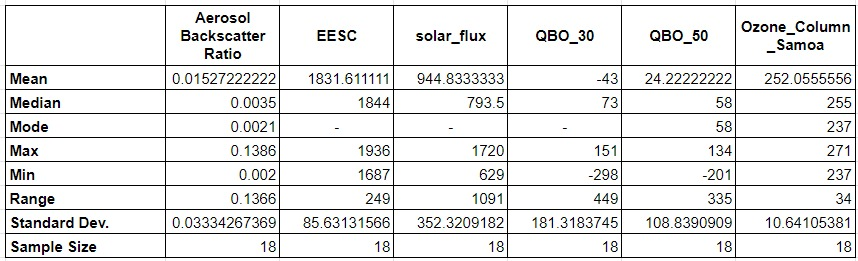
\includegraphics[scale=0.45]{src/Pics/SamoApril.jpeg}
    \caption{Tabel Analisis Deskriptif Untuk Samoa - April}
    \label{fig:my_label}
\end{figure}
Pada Baris Mode dapat terlihat bahwa EESC, Solar Flux, dan QBO 30 tidak memiliki nilai yang terulang sehingga pada tabel diberikan garis.
%-----------------------------------------------------------------------------%
\section{Pemodelan}
%-----------------------------------------------------------------------------%
Bagian ini akan menjelaskan pemodelan yang telah kami lakukan untuk analisis faktor-faktor pengaruh variasi konsentrasi lapisan ozon.

\subsection{Alur Pemodelan}
Secara garis besar, alur dari proses pemodelan yang telah dilakukan adalah sebagai berikut.
\begin{enumerate}
    \item Seleksi Variabel dan Estimasi Parameter
    \item Pemeriksaan Asumsi Error
    \item Penilaian Kelayakan Model
\end{enumerate}
Tahapan-tahapan di atas akan dijelaskan lebih lanjut dan disertakan dengan hasilnya di bagian-bagian selanjutnya.
\\~\\
Untuk memberikan gambaran akan alur pemodelan yang dilakukan, kami akan membahas alur untuk pemodelan daerah Samoa pada Bulan April. Proses pemodelan untuk bulan dan daerah lain adalah sama, sehingga kami hanya akan merangkum hasilnya di bagian \ref{hasil pemodelan}.
\subsection{Seleksi Variabel dan Estimasi Parameter}
Pada tahapan ini, kami mencari variabel-variabel yang layak untuk digunakan pada model. Hal pertama yang kami periksa adalah multikolinearitas. Multikolinearitas adalah penyelidikan ada atau tidaknya indikasi hubungan linear antara variabel-variabel penjelas. Nilai multikolinearitas yang tinggi mengindikasikan adanya beberapa variabel yang mengandung informasi yang sama. Hal ini dapat mengurangi kemampuan interpretasi model. Sebab, ini artinya variabel penjelasnya tidak independen satu dengan yang lain.
\\~\\
Uji multikolinearitas dapat dilakukan dengan berbagai cara, antara lain dengan matriks korelasi dan \textit{Variance Inflation Factor} (VIF). Karena jumlah variabel penjelas tidak terlalu banyak, kita akan menggunakan matriks korelasi.
\begin{figure}[h!]
    \centering
    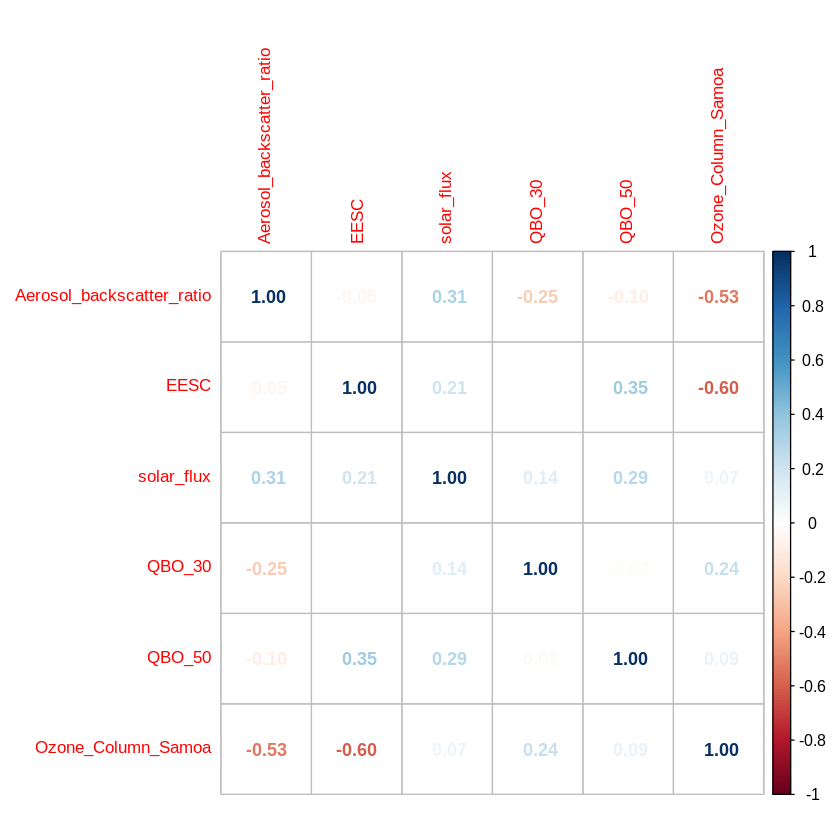
\includegraphics[scale=0.5]{src/Pics/corrmatrix.png}
    \caption{Matriks Korelasi antar Variabel Untuk Samoa - April}
    \label{fig:my_label}
\end{figure}
Dari matriks korelasi diatas, terlihat bahwa tidak ada variabel penjelas yang memiliki korelasi Pearson kuat. Artinya, tidak ada indikasi multikolinearitas dari data variabel penjelas kita. Jadi, kita dapat menggunakan semua variabel yang ada.
\\~\\
Setelah memeriksa multikolinearitas, seleksi variabel dilanjutkan dengan \textit{stepwise regression}. Model yang akan kita ajukan adalah model dengan interaksi orde 2. Dengan kata lain, model terluas yang mungkin adalah sebagai berikut.
\begin{align*}
    Y = &\beta_0 + \beta_1X_1 + \beta_2X_2 + \beta_3X_3 + \beta_4X_4 + \beta_5X_5 + \beta_6X_1X_2 + \beta_7X_1X_3 + \beta_8X_1X_4 + \beta_9X_1X_5\\
    &+ \beta_{10}X_2X_3 + \beta_{11}X_2X_4 + \beta_{12}X_2X_5 + \beta_{13}X_3X_4 + \beta_{14}X_3X_5 + \beta_{15}X_4X_5 + \epsilon,\;\epsilon \sim N(0, \sigma^2)
\end{align*}
Berikut adalah representasi variabel yang digunakan pada persamaan di atas.
\begin{enumerate}
    \item $X_1:$ Aerosol\_backscatter\_ratio
    \item $X_2:$ EESC
    \item $X_3:$ solar\_flux
    \item $X_4:$ QBO\_30
    \item $X_5:$ QBO\_50
    \item $Y\;\: :$ Ozone\_Column\_Samoa
\end{enumerate}
Model tersebut adalah model yang lumayan besar dengan 16 derajat kebebasan. \textit{Stepwise regression} akan menyeleksi variabel-variabel yang paling berpengaruh.
\\~\\
Setelah menjalankan \textit{stepwise regression}, berikut adalah hasil yang kami dapatkan.\\
\begin{figure}[h!]
    \centering
    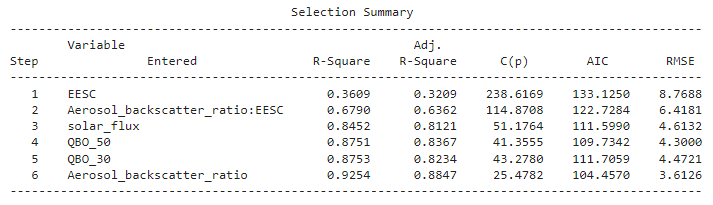
\includegraphics[scale=0.9]{src/Pics/stepwiseregress.png}
    \caption{\textit{Printout} Hasil \textit{Stepwise Regression} di R}
    \label{fig:my_label}
\end{figure}\\
Pada tabel tersebut, kolom \textit{step} menunjukkan nomor iterasi. Variabel-variabel yang dimasukkan ke dalam model pada setiap step dituliskan pada kolo\textit{entered}. Kolom-kolom lainnya merupakan statistik-statistik untuk model-model yang dibangun pada setiap\textit{step}, yaitu $R^2$, \textit{adjusted} $R^2$, Mallow's $C_p$, Akaike Information Criterion (AIC), serta RMSE.  Makna dari masing-masing statistik tersebut sesuai dengan yang telah dijelaskan pada bagian \ref{Statistik Model Regresi}. Kita menggunakan hasil\textit{stepwise regression} untuk membangun model pertama kita. Dalam bentuk persamaan, model pertama kita dapat dituliskan dengan persamaan berikut.
\begin{equation*}
    Y = \beta_0 + \beta_1X_1 + \beta_2X_2 + \beta_3X_3 + \beta_4X_4 + \beta_5X_5 + \beta_6X_1X_2 +\epsilon,\;\epsilon \sim N(0, \sigma^2)
\end{equation*}
Model diatas akan kita sebut sebagai \textbf{model 1}. Kita dapat menjalankan algoritma regresi \textit{Ordinary Least Squares} untuk mencari taksiran dari koefisien-koefisien regresi $\beta_i$. Berikut adalah hasilnya.
\begin{figure}[h!]
    \centering
    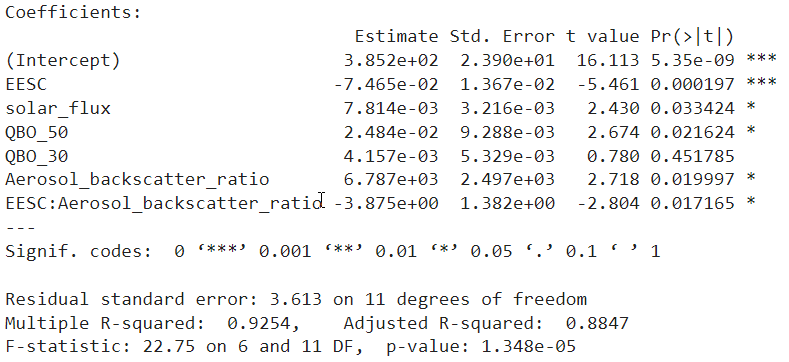
\includegraphics[scale=0.7]{src/Pics/firstfitting.png}
    \caption{\textit{Printout} Hasil \textit{Fitting} model 1 di R}
    \label{fig:my_label}
\end{figure}\\
Pada gambar di atas, nilai taksiran untuk koefisien-koefisien regresi diberikan pada kolom \textit{Estimate}.
\\~\\
Kolom $Pr(>|t|)$ adalah nilai probabilitas yang digunakan untuk uji-t masing-masing variabel. Perhatikan bahwa $X_4$ tidak memenuhi uji-t. Oleh karena itu, kita akan mencoba menghilangkan variabel tersebut dan melakukan \textit{fitting} dengan model berikut.
\begin{equation*}
    Y = \beta_0 + \beta_1X_1 + \beta_2X_2 + \beta_3X_3 + \beta_4X_5 + \beta_5X_1X_2 +\epsilon,\;\epsilon \sim N(0, \sigma^2)
\end{equation*}
Model ini akan kita sebut sebagai Model 2. Hasil dari prosses \textit{fitting} dengan R adalah sebagai berikut.
\begin{figure}[h!]
    \centering
    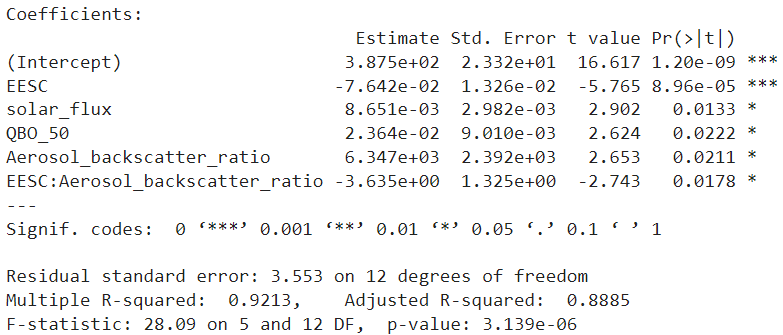
\includegraphics[scale=0.7]{src/Pics/secondfitting.png}
    \caption{\textit{Printout} Hasil \textit{Fitting} model 2 di R}
    \label{fig:model2}
\end{figure}\\
\subsection{Pemeriksaan Asumsi Error}
Setelah kita telah mendapatkan model, yaitu model 2, kita memeriksa apakah model kita memenuhi asumsi-asumsi error dalam regresi biasa. Pemeriksaan asumsi penting untuk memastikan bahwa model kita merupakan model yang baik, sehingga kita dapat menginterpretasikan model dengan tepat. Asumsi-asumsi error yang digunakan dalam regresi biasa adalah sebagai berikut.
\begin{enumerate}
    \item Mean dari error adalah 0.
    \item Error berdistribusi normal 
    \item Homoskedastisitas error
    \item Independensi error
\end{enumerate}
Untuk memeriksa keempat kriteria berikut, kita akan menggambar berbagai grafik yang mengandung nilai-nilai residual dari model kita.
\\~\\
Pertama, kita akan melihat grafik dari \textit{residual vs fitted}. Sumbu $x$ dari grafik ini adalah nilai-nilai data dari variabel dependen, yaitu $y_i$. Sedangkan sumbu $y$ dari grafik ini adalah residual untuk setiap $y_i$, yaitu $\hat{y_i}-y_i$.\\
\begin{figure}[h!]
    \centering
    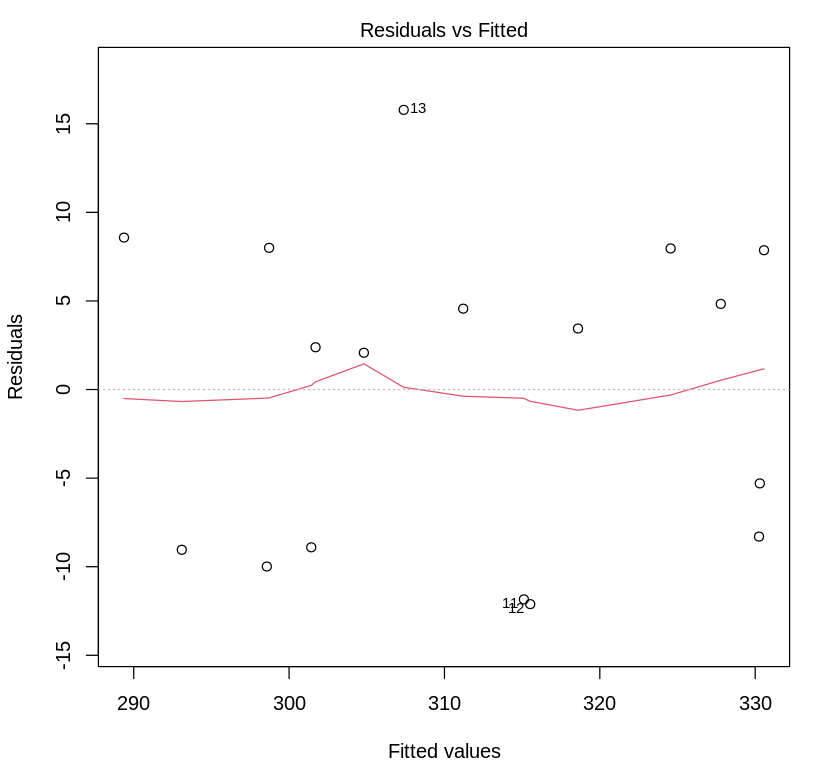
\includegraphics[scale=0.5]{src/Pics/res vs fitted.png}
    \caption{\textit{Printout} Grafik \textit{Residual vs Fitted} untuk Model 2}
    \label{fig:res vs fitted}
\end{figure}~\\
Dari grafik diatas, terlihat bahwa mean dari residual adalah 0. Ini mengindikasikan bahwa asumsi pertama kita terpenuhi, yaitu mean dari error adalah 0.
\\~\\
Untuk memeriksa bahwa distribusi dari error adalah normal, kita dapat menggunakan grafik \textit{Q-Q}.\\
\begin{figure}[h!]
    \centering
    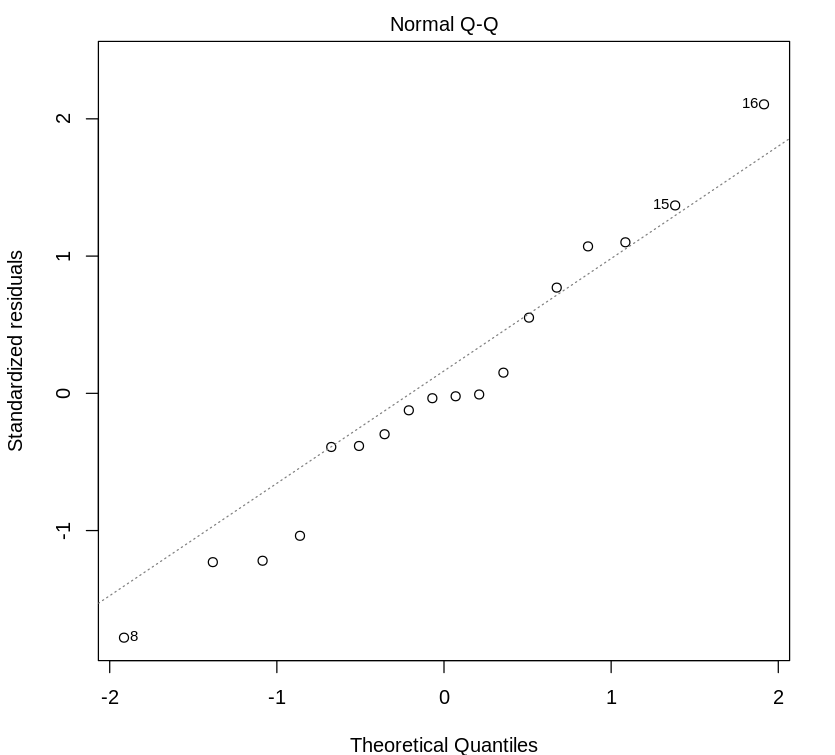
\includegraphics[scale=0.5]{src/Pics/normality.png}
    \caption{\textit{Printout} Grafik \textit{Q-Q} untuk Model 2}
\end{figure}~\\
Pada grafik tersebut, jika distribusi error normal, titik-titik pada grafik akan terletak pada garis. Posisi titik-titik yang mendekati garis menunjukkan bahwa distribusi dari residual mendekati distribusi normal. Ini merupakan indikasi bahwa error dari model 2 mendekati distribusi normal. Secara umum error yang tidak sepenuhnya mengikuti distribusi normal tidak terlalu memengaruhi regresi. Oleh karena itu, kami akan menganggap bahwa asumsi kedua sudah cukup terpenuhi.
\\~\\
Untuk memeriksa homoskedastisitas error, kita akan menggunakan grafik \textit{Scale-Location}. Grafik ini menunjukkan nilai akar dari residual setelah standarisasi terhadap nilai $y_i$. Garis yang mengikuti garis lurus mengindikasikan bahwa asumsi homoskedastisitas terpenuhi.\\
\begin{figure}[h!]
    \centering
    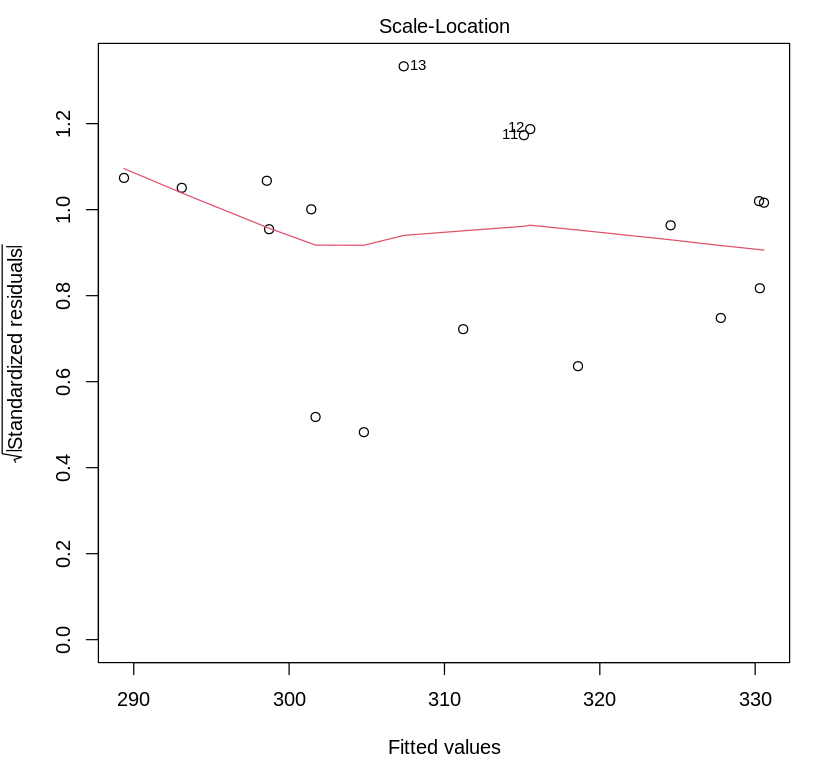
\includegraphics[scale=0.5]{src/Pics/homoscedasticity.png}
    \caption{\textit{Printout} Grafik \textit{Scale-Location} untuk Model 2}
\end{figure}
\\~\\
Terakhir, kita dapat memeriksa asumsi independensi error dengan grafik \textit{residual vs fitted} pada bagian sebelumnya. Error yang dependen akan membentuk suatu pola, umumnya sebuah periodisitas. Terlihat bahwa pada grafik tersebut nilai residual tidak membentuk pola apapun. Ini adalah indikasi bahwa error independen satu dengan yang lain.
\subsection{Penilaian Kelayakan Model}
Pada bagian ini, kita akan menilai performa model dengan statistik $R^2$. Pada gambar \ref{fig:model2}, kita memperoleh nilai $R^2 = 0.9213$. Artinya, sekitar $92\%$ variabilitas dari nilai variabel dependen dapat dijelaskan oleh model. Nilai ini merupakan akurasi yang baik.

\subsection{Analisis Koefisien Regresi}
Pada gambar \ref{fig:model2} kolom \textit{estimate} merupakan kolom estimasi parameter koefisien regresinya untuk setiap variabel \textit{proxy}. Nilai estimasi positif menandakan bahwa kenaikkan nilai variabel \textit{proxy} tersebut akan menyebabkan kenaikkan nilai dari \textit{total column ozone}. sebaliknya, nilai estimasi yang negatif menandakkan bahwa kenaikkan nilai dari variabel \textit{proxy}, akan  menyebabkan penurunan nilai dari \textit{total column ozone}. Selain itu, perlu diingat bahwa \textit{magnitude} dari koefisien regresi tersebut tidak dapat kita bandingkan karena pada proses pemodelan, kita tidak melakukan normalisasi data.

Tabel berikut merangkum  efek-efek variabel  \textit{proxy} terhadap \textit{total column ozone} pada daerah tropis di bulan April .
\begin{table}[!ht]
    \centering
    \begin{tabular}{|l|l|}
    \hline
        Variabel proxy & Efek variabel terhadap Total Column Ozone \\ \hline
        EESC  & Berbanding terbalik \\ \hline
        QBO-30 & Tidak signifikan \\ \hline
        QBO-50 & Berbanding lurus\\ \hline
        Solar Flux & Berbanding lurus\\ \hline
        Aerosol backscatter ratio & Berbanding lurus\\ \hline
    \end{tabular}
\end{table}

%-----------------------------------------------------------------------------%
\section{Hasil Pemodelan}\label{hasil pemodelan}
%-----------------------------------------------------------------------------%

\subsection{Rangkuman Hasil Pemodelan}
Bagian berikut adalah rangkuman (berupa tabel) mengenai hasil pemodelan untuk setiap daerah observasi (tabel dibagi per daerah  observasi, terdapat 5 tabel). Kolom dari tabel menunjukkan variabel \textit{proxy} dan baris dari tabel menunjukkan bulan (Januari hingga Desember). sebuah ceklis pada tabel menandakan bahwa variabel \textit{proxy} tersebut lolos uji-t (uji signifikansi dengan distribusi t) untuk bulan yang bersesuaian. Variabel \textit{proxy} yang  lolos uji t berarti variabel \textit{proxy} tersebut dapat menjelaskan variabilitas dari \textit{total column ozone} pada daerah observasinya untuk bulan yang bersesuainnya. Halaman berikut merupakan rangkuman dari tabel yang dimaksud.

\begin{table}[p]

\begin{tabular}{|l|l|l|l|l|l|l|}
\hline Tropis & EESC & QBO-30 & QBO-50 & SolarFlux & Aerosol backscatter \\
\hline Jan & $\checkmark$ & $\mathbf{x}$ & $\mathbf{x}$ & $\mathbf{x}$ & $\mathbf{x}$ \\
\hline Feb & $\mathbf{x}$ & $\mathbf{x}$ & $\mathbf{x}$ & $\mathbf{x}$ & $\mathbf{x}$ \\
\hline Mar & $\checkmark$ & $\mathbf{x}$ & $\mathbf{x}$ & $\mathbf{x}$ & $\checkmark$ \\
\hline Apr & $\checkmark$ & $\mathbf{x}$ & $\checkmark$ & $\checkmark$ & $\checkmark$ \\
\hline May & $\checkmark$ & $\mathbf{x}$ & $\mathbf{x}$ & $\mathbf{x}$ & $\checkmark$ \\
\hline Jun & $\checkmark$ & $\mathbf{x}$ & $\mathbf{x}$ & $\mathbf{x}$ & $\checkmark$ \\
\hline Jul & $\checkmark$ & $\mathbf{x}$ & $\mathbf{x}$ & $\mathbf{x}$ & $\checkmark$ \\
\hline Aug & $\checkmark$ & $\mathbf{x}$ & $\mathbf{x}$ & $\mathbf{x}$ & $\mathbf{x}$ \\
\hline Sep & $\mathbf{x}$ & $\mathbf{x}$ & $\mathbf{x}$ & $\mathbf{x}$ & $\mathbf{x}$ \\
\hline Oct & $\mathbf{x}$ & $\mathbf{x}$ & $\mathbf{x}$ & $\mathbf{x}$ & $\mathbf{x}$ \\
\hline Nov & $\mathbf{x}$ & $\mathbf{x}$ & $\mathbf{x}$ & $\mathbf{x}$ & $\mathbf{x}$ \\
\hline Dec & $\mathbf{x}$ & $\mathbf{x}$ & $\mathbf{x}$ & $\mathbf{x}$ & $\mathbf{x}$ \\
\hline
\end{tabular}

    \caption{Rangkuman Hasil Pemodelan Pada Daerah Tropis}
    \label{tab:tropis}
\end{table}


\begin{table}[p]
    \centering

    \begin{tabular}{|l|l|l|l|l|l|l|}
\hline Subtropis (S) & EESC & QBO-30 & QBO-50 & SolarFlux & Aerosol backscatter \\
\hline Jan & $\mathbf{x}$ & $\mathbf{x}$ & $\mathbf{x}$ & $\mathbf{x}$ & $\mathbf{x}$ \\
\hline Feb & $\mathbf{x}$ & $\mathbf{x}$ & $\mathbf{x}$ & $\mathbf{x}$ & $\mathbf{x}$ \\
\hline Mar & $\mathbf{x}$ & $\mathbf{x}$ & $\mathbf{x}$ & $\mathbf{x}$ & $\mathbf{x}$ \\
\hline Apr & $\mathbf{x}$ & $\mathbf{x}$ & $\mathbf{x}$ & $\mathbf{x}$ & $\mathbf{x}$ \\
\hline May & $\mathbf{x}$ & $\mathbf{x}$ & $\mathbf{x}$ & $\mathbf{x}$ & $\mathbf{x}$ \\
\hline Jun & $\checkmark$ & $\checkmark$ & $\mathbf{x}$ & $\mathbf{x}$ & \checkmark \\
\hline Jul & $\checkmark$ & $\checkmark$ & $\mathbf{x}$ & $\mathbf{x}$ & $\mathbf{x}$ \\
\hline Aug & $\checkmark$ & $\checkmark$ & $\mathbf{x}$ & $\mathbf{x}$ & $\mathbf{x}$ \\
\hline Sep & $\checkmark$ & $\checkmark$ & $\mathbf{x}$ & $\mathbf{x}$ & $\mathbf{x}$ \\
\hline Oct & $\checkmark$ & $\checkmark$ & $\mathbf{x}$ & $\mathbf{x}$ & $\mathbf{x}$ \\
\hline Nov & $\mathbf{x}$ & $\mathbf{x}$ & $\mathbf{x}$ & $\mathbf{x}$ & $\mathbf{x}$ \\
\hline Dec & $\mathbf{x}$ & $\mathbf{x}$ & $\mathbf{x}$ & $\mathbf{x}$ & $\mathbf{x}$ \\
\hline
\end{tabular}
    
    \caption{Rangkuman Pemodelan Daerah Subtropis Selatan}
    \label{tab:subtropisS}
\end{table}


\begin{table}[p]
    \centering

\begin{tabular}{|l|l|l|l|l|l|}
\hline Subtropis (N) & EESC & QBO-30 & QBO-50 & SolarFlux & Aerosol backscatter \\
\hline Jan & $\mathbf{x}$ & $\checkmark$ & $\mathbf{x}$ & $\mathbf{x}$ & $\mathbf{x}$ \\
\hline Feb & $\mathbf{x}$ & $\mathbf{x}$ & $\mathbf{x}$ & $\mathbf{x}$ & $\mathbf{x}$ \\
\hline Mar & $\mathbf{x}$ & $\mathbf{x}$ & $\mathbf{x}$ & $\mathbf{x}$ & $\mathbf{x}$ \\
\hline Apr & $\mathbf{x}$ & $\mathbf{x}$ & $\mathbf{x}$ & $\mathbf{x}$ & $\mathbf{x}$ \\
\hline May & $\mathbf{x}$ & $\mathbf{x}$ & $\mathbf{x}$ & $\mathbf{x}$ & $\mathbf{x}$ \\
\hline Jun & $\mathbf{x}$ & $\mathbf{x}$ & $\mathbf{x}$ & $\mathbf{x}$ & $\mathbf{x}$ \\
\hline Jul & $\mathbf{x}$ & $\mathbf{x}$ & $\mathbf{x}$ & $\mathbf{x}$ & $\mathbf{x}$ \\
\hline Aug & $\mathbf{x}$ & $\mathbf{x}$ & $\mathbf{x}$ & $\mathbf{x}$ & $\mathbf{x}$ \\
\hline Sep & $\mathbf{x}$ & $\mathbf{x}$ & $\mathbf{x}$ & $\mathbf{x}$ & $\mathbf{x}$ \\
\hline Oct & $\mathbf{x}$ & $\mathbf{x}$ & $\mathbf{x}$ & $\mathbf{x}$ & $\mathbf{x}$ \\
\hline Nov & $\mathbf{x}$ & $\mathbf{x}$ & $\mathbf{x}$ & $\mathbf{x}$ & $\mathbf{x}$ \\
\hline Dec & $\mathbf{x}$ & $\mathbf{x}$ & $\mathbf{x}$ & $\mathbf{x}$ & $\mathbf{x}$ \\
\hline
\end{tabular}

    \caption{Rangukuman Pemodelan Daerah Subtropis Utara}
    \label{tab:subtropisN}
\end{table}

\begin{table}[p]
    \centering
\begin{tabular}{|l|l|l|l|l|l|l|}
\hline Polar (N) & EESC & QBO-30 & QBO-50 & SolarFlux & Aerosol backscatter & AB : EESC \\
\hline Jan & $x$ & $x$ & $x$ & $x$ & $x$ & $x$ \\
\hline Feb & $x$ & $x$ & $x$ & $x$ & $x$ & $x$ \\
\hline Mar & $x$ & $x$ & $x$ & $x$ & $x$ & $x$ \\
\hline Apr & $x$ & $x$ & $x$ & $x$ & $x$ & $x$ \\
\hline May & $x$ & $x$ & $x$ & $x$ & $x$ & $x$ \\
\hline Jun & $\checkmark$ & $x$ & $\checkmark$ & $x$ & $\checkmark$ & $\checkmark$ \\
\hline Jul & $\checkmark$ & $x$ & $\checkmark$ & $x$ & $\checkmark$ & $x$ \\
\hline Aug & $x$ & $x$ & $x$ & $x$ & $x$ & $x$ \\
\hline Sep & $x$ & $x$ & $x$ & $x$ & $x$ & $x$ \\
\hline Oct & $x$ & $x$ & $x$ & $x$ & $x$ & $x$ \\
\hline Nov & $x$ & $x$ & $x$ & $x$ & $x$ & $x$ \\
\hline Dec & $x$ & $x$ & $x$ & $x$ & $x$ & $x$ \\
\hline
\end{tabular}

    \caption{Rangkuman Pemodelan Daerah Kutub Utara}
    \label{tab:NP}
\end{table}

\begin{table}[p]
    \centering


\begin{tabular}{|l|l|l|l|l|l|}
\hline Polar (S) & EESC & QBO-30 & QBO-50 & SolarFlux & Aerosol backscatter \\
\hline Jan & $\mathbf{x}$ & $\mathbf{x}$ & $\mathbf{x}$ & $\mathbf{x}$ & $\mathbf{x}$ \\
\hline Feb & $\mathbf{x}$ & $\mathbf{x}$ & $\mathbf{x}$ & $\mathbf{x}$ & $\mathbf{x}$ \\
\hline Mar & $\checkmark$ & $\mathbf{x}$ & $\mathbf{x}$ & $\mathbf{x}$ & $\checkmark$ \\
\hline Apr & $\mathbf{x}$ & $\mathbf{x}$ & $\checkmark$ & $\mathbf{x}$ & $\checkmark$ \\
\hline May & $\mathbf{x}$ & $\mathbf{x}$ & $\mathbf{x}$ & $\mathbf{x}$ & $\mathbf{x}$ \\
\hline Jun & $\mathbf{x}$ & $\mathbf{x}$ & $\mathbf{x}$ & $\mathbf{x}$ & $\mathbf{x}$ \\
\hline Jul & $\mathbf{x}$ & $\mathbf{x}$ & $\mathbf{x}$ & $\mathbf{x}$ & $\mathbf{x}$ \\
\hline Aug & $\mathbf{x}$ & $\mathbf{x}$ & $\mathbf{x}$ & $\mathbf{x}$ & $\mathbf{x}$ \\
\hline Sep & $\mathbf{x}$ & $\mathbf{x}$ & $\mathbf{x}$ & $\mathbf{x}$ & $\mathbf{x}$ \\
\hline Oct & $\mathbf{x}$ & $\mathbf{x}$ & $\mathbf{x}$ & $\mathbf{x}$ & $\mathbf{x}$ \\
\hline Nov & $\mathbf{x}$ & $\mathbf{x}$ & $\mathbf{x}$ & $\mathbf{x}$ & $\mathbf{x}$ \\
\hline Dec & $\mathbf{x}$ & $\mathbf{x}$ & $\mathbf{x}$ & $\mathbf{x}$ & $\mathbf{x}$ \\
\hline
\end{tabular}



    \caption{Rangkuman Pemodelan Daerah Kutub Selatan}
    \label{tab:SP}
\end{table}



\subsection{Interpretasi}

Pada daerah tropis, variabel \textit{proxy} EESC adalah variabel terbaik  yang menjelaskan variabilitas \textit{total column ozone} karena dapat terlihat bahwa pada tabel \ref{tab:tropis}, variabel EESC dapat menjelaskan variabilitas \textit{total column ozone} 7 dari 12 bulan. Selanjutnya, variabel \textit{proxy} \textit{aerosol backcatter ratio} dapat menjelaskan variabilitas \textit{total column ozone} 5 dari 12 bulan. Variabel \textit{proxy} QBO-30, QBO-50, Solar Flux tidak dapat menjelaskan variabilitas \textit{total column ozone}.

Pada Daerah subtropis Selatan, variabel \textit{proxy} QBO-30 dan EESC adalah variabel proxy terbaik untuk menjelaskan variabilitas \textit{total column ozone} (dengan total 5 dari 12 bulan terjelaskan dengan kedua variabel proxy). Namun, pada daerah subtropis utara, tidak ada variabel \textit{proxy} yang menjelaskan dengan baik variabilitas \textit{total column ozone}.

Pada daerah kutub, secara general tidak ada variabel \textit{proxy} yang menjelaskan variabilitas \textit{total column ozone} diatas dua bulan. Temuan unik adalah variabel interaksi antara \textit{aerosol backscatter ratio} dengan EESC (orde 2 regresi) dapat menjelaskan variabilitas \textit{total column ozone} di kutub selatan pada bulan Juni, dan Juli. 





%-----------------------------------------------------------------------------%
\chapter{Penutup}
%-----------------------------------------------------------------------------%



%-----------------------------------------------------------------------------%
\section{Kesimpulan}
Dari hasil pengujian bab 2.5, dapat dilihat bahwa  tidak semua variabel \textit{proxy}  dapat menjelaskan variabilitas \textit{total colummn ozone} di setiap garis daerah (tropis, subtropis selatan, subtropis utara, kutub utara, kutub selatan). Pada daerah tropis, ditemukan bahwa variabel \textit{proxy} EESC dan \textit{aerosol backscatter ratio} adalah variabel \textit{proxy} yang dapat menjelaskan variabilitas TCO dengan baik. Di lain sisi, pada daerah subtropis selatan, EESC dan QBO-30 lah merupaka variabel penjelas yang baik. Namun, pada daerah subtropis utara, kutub selatan, kutub utara, tidak ditemukan variabel \textit{proxy} yang dapat menjelaskan variabilitas total column ozone dengan baik. 
%-----------------------------------------------------------------------------%

%-----------------------------------------------------------------------------%
\section{Saran}
Proses pembentukan dan penghancuran  lapisan ozon merupakan proses yang dinamik dan rumit. Kelima variabel \textit{proxy} yang digunakan belum dapat meng-\textit{capture} semua proses dinamik tersebut secara global. Oleh karena itu, pada penelitian selanjutnya, kami dapat mempertimbangkan variabel-variabel \textit{[proxy} lainnya, sehingga  memperluas ukuran model. Dengan begitu, kami harapkan bahwa performa model akan jauh lebih baik. Selain itu, rentang waktu tahun  (derajat bebas) dari  model juga dapat  diperpanjang, sehingga kami harapkan juga performa model yang lebih baik.
%-----------------------------------------------------------------------------%



%Daftar Pustaka
\begin{thebibliography}{}
\bibitem{stat-regression}
Mendenhall, William & Sincich, Terry. (1997). A Second Course in Statistics: Regression Analysis. Journal of the American Statistical Association. 92. 10.2307/2965740. 

\bibitem{ozone-assesment}
WMO (World Meteorological Organization), Scientific Assessment of Ozone Depletion: 2018, Global Ozone Research and Monitoring Project – Report No. 58, 588 pp., Geneva, Switzerland, 2018.

\bibitem{process-based}
Wohltmann, I., Rex, M., Brunner, D., M ̈ader, J.. (2005). Integrated equivalent latitude as a proxy for dynamical changes in ozone column. Geophysical Research Letters. 3210. 1029/2005GL022497.​
\bibitem{EESC-ref}
Newman, P. A., Daniel, J. S., Waugh, D. W., and Nash, E. R.. A new formulation of equivalent effective stratospheric chlorine (EESC), Atmos. Chem. Phys., 7, 4537–4552, https://doi.org/10.5194/acp-7-4537-2007, 2007.

\bibitem{trend-NP}
Bojkov, R. D., L. Bishop, W. J. Hill, G. C. Reinsel, and G. C. Tiao (1990), A statistical trend analysis of revised Dobson total ozone data over the northern hemisphere, J. Geophys. Res., 95, 9785–9807.

\bibitem{dynamic-proxy}
Ziemke, J., S. Chandra, R. McPeters, and P. Newman (1997), Dynamical proxies of column ozone with applications to global trend models, J. Geophys. Res., 102(D5), 6117– 6129.

\bibitem{bolder}
CLUE: Chemistry, Life, the Universe, and Everything. (2022, April 3). Michigan State University and UC Bolder.https://chem.libretexts.org/@go/page/354112

\bibitem{brute-force}
Mäder, J. A., Staehelin, J., Brunner, D., Stahel, W. A., Wohltmann, I., and Peter, T. (2007), Statistical modeling of total ozone: Selection of appropriate explanatory variables, J. Geophys. Res., 112, D11108, doi:10.1029/2006JD007694.

\bibitem{data-set}
Halogen Chemistry dataset reference:\\
https://gml.noaa.gov/dv/data.html\\
https://agage.mit.edu/data/agage-data\\
https://gml.noaa.gov/hats/odgi.html\\

\bibitem{dataset-2}
QBO dataset reference:\\
https://www.geo.fuberlin.de/en/met/ag/strat/produkte/qbo/index.html

\bibitem{dataset-3}
Heterogeneous Polar Chemistry dataset reference\\
https://openbooks.lib.msu.edu/clue/chapter/chapter-4-heterogeneous-compounds/

\bibitem{data-set-4}
Aerosol dataset reference:\\
https://data.giss.nasa.gov/modelforce/strataer//tau.line$_$2012.12.txt

\bibitem{data-set-5}
Solar Cycle dataset reference:\\ 
https://www.ngdc.noaa.gov/stp/space-weather/solar-data/solar-features/solar-radio/
 
\end{thebibliography}

% Alternatif manajemen daftar pustaka dengan \bibliography

%
% Lampiran 
%
% \begin{appendix}
% 	%
% @author  Andreas Febrian
% @version 1.00 
% 
% Hanya sebuah pembatas bertuliskan LAMPIRAN ditengah halaman. 
% 

\begin{titlepage}
	\centering 
	\vspace*{6cm}
	\noindent \Huge{LAMPIRAN}
	\addChapter{LAMPIRAN}
\end{titlepage}
% 	\setcounter{page}{2}\textbf{}
% 	%-----------------------------------------------------------------------------%
\addChapter{Lampiran 1}
\chapter*{Lampiran 1}
%-----------------------------------------------------------------------------%
% \end{appendix}

\end{document}